\chapter{Results}
\label{ch:results}

\Cref{fig:model} plots the model from \cref{eq:model} with the parameters of
\cref{tab:params}. A summary chart is shown in \cref{fig:chart}.

\begin{figure}[htbp]
  \centering
  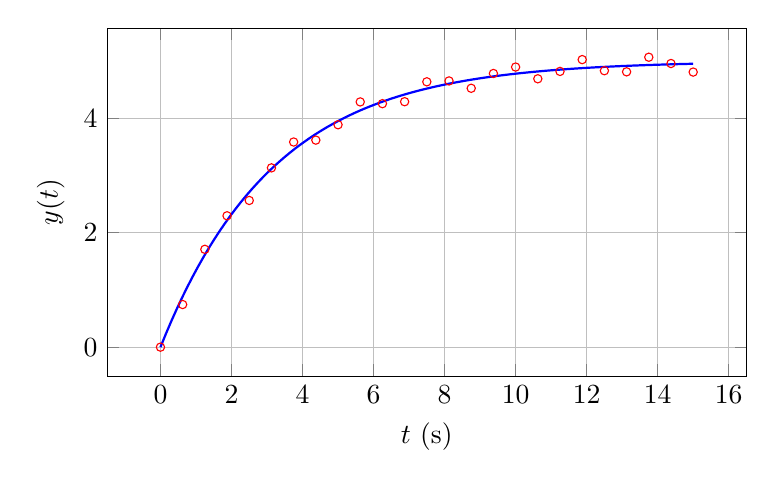
\begin{tikzpicture}
    \begin{axis}[width=0.8\linewidth, height=6cm, xlabel={$t$ (s)}, ylabel={$y(t)$}, grid=major, domain=0:15, samples=100]
      \addplot[thick, blue] {5*(1-exp(-x/3.2))};
      \addplot[only marks, mark=o, mark size=1.5pt, samples=25, red] {5*(1-exp(-x/3.2)) + 0.15*sin(deg(7*x))};
    \end{axis}
  \end{tikzpicture}
  \caption{Model curve and simulated measurements.}
  \label{fig:model}
\end{figure}

\begin{figure}[htbp]
  \centering
  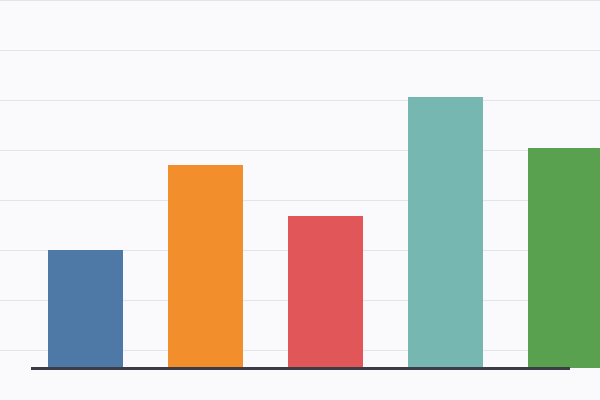
\includegraphics[width=0.55\linewidth]{chart.png}
  \caption{A raster image of a bar chart.}
  \label{fig:chart}
\end{figure}
